\chapter{Systemarkitektur}
Systemarkitekturen har til formål at beskrive både hardware- og softwarekomponenter til sådan en grad at sammensætningen af hele system kan forstås. I dette afsnit beskrives arkitektur for både hardware og software.

I hardwarearkitekturen beskrives systemet ved at nedbryde det i blokke. I BDD'et er blokkenes porte og associationer til andre blokke angivet. Disse porte anvendes senere i afsnittet, hvor de benyttes i IBD'et.

I softwarearkitekturen udarbejdes der applikationsmodeller bestående af sekvensdiagrammer og klassediagrammer for hver use case, opdelt for hver CPU i systemet. Applikationsmodellerne har til formål at danne et overblik af de krav der stilles til softwaren for produktets uses cases. På denne måde kan de bruges som inspirerende grundlæg for software design og implementering. Applikationsmodellerne giver en overfladisk beskrivelse af CPU'ernes interaktioner.

\section{Domæne model}
På figur \ref{fig:DomainModel} ses domæne modellen for systemet. Denne er lavet for at danne et overblik over systemet, og hvordan de forskellige dele overfladisk interagerer med hinanden. 

\begin{figure}[H]
	\centering
	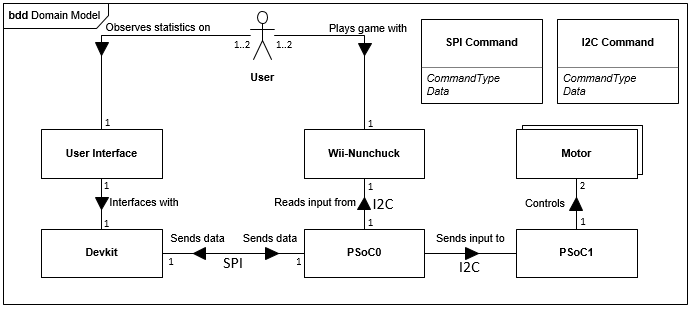
\includegraphics[width=\textwidth]{Systemarkitektur/images/DomainModel}
	\caption{Domæne model for Candygun 3000}
	\label{fig:DomainModel}
\end{figure}

I domæne modellen ses, at brugeren interagerer med både Wii-nunchucken og med brugergrænsefladen. Brugergrænsefladen er en grænseflade til softwaren devkittet. Devkittet kommunikerer med PSoC0, som læser den analoge data der kommer fra Wii-nunchucken. Denne data bliver derefter afkodet og videresendt til PSoC1, som styrer motorene ud fra dataene.

I "I2C Command" ses en grov estimering af interfacet mellem de forskellige I2C enheder i systemet. Commandtype bruges til at identificere hvilken data der bliver sendt. Data er en mængde tal-værdier der bliver tolket ud fra hvilken commandtype der er blevet sendt.

I "SPI Command" ses en estimering af interfacet mellem SPI enhederne i systemet. "Commandtype" bruges til at identificere hvilken opgave systemet skal udføre (f.eks. 'I2C-test'). Data kan indeholde tal-værdier, som repræsenterer nunchuck værdier (buttonpress osv.). 
En mere detaljeret gennemgang af disse kommunikations protokoller kan findes i afsnit \ref{afsnit:kommunikationsprotokoller} - Kommunikationsprotokoller.

% ---------------BDD--------------------------------------------------
\section{BDD for Candygun 3000}
På figur \ref{fig:BDD} ses et \textit{Block Definition Diagram (BDD)} hvor Candygun 3000 brudt ned i blokkene PSoC0, PSoC1 og Devkit 8000. Devkit 8000 er brugergrænsefladen, som brugeren kan interagere med via touchskærmen. Denne kommunikerer via SPI til PSoC0, som er SPI-slave. PSoC0 er forbundet til PSoC1, hvor kommunikeres via I2C og den fungerer som I2C-master. Udover bindeled mellem SPI og I2C kommunikationen har  PSoC0 ansvaret for Wii-nunchucken. PSoC1 står for ar aflæse og afkode input fra nunchucken, som også kommunikerer via I2C, og videresender dataene til PSoC1. PSoC1, som står for motorstyringen, tager dataene og konverterer dem til et PWM-signal. Dette signal sendes derefter til de to motorer. På figur \ref{fig:BDD} ses blokkenes associationer og deres porte.  

\begin{figure}[H]
	\centering
	%trim = {1.8cm 14.6cm 1.8cm 1cm}, clip = true, %
	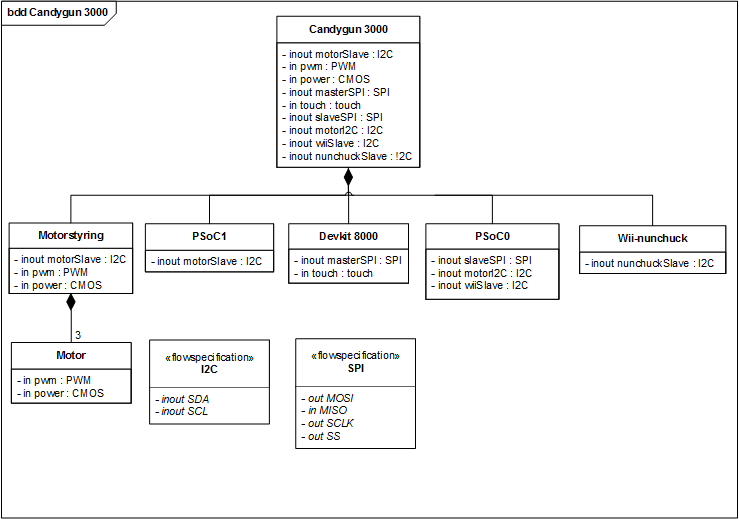
\includegraphics[width= \textwidth]{Systemarkitektur/images/BDD_overordnet.png}
	\caption{BDD for Candygun 3000}
	\label{fig:BDD}
\end{figure}


\subsection{Blokbeskrivelse}
Følgende afsnit indeholder en blokbeskrivelse samt en flowspecifikation for I2C og SPI. I flowspecifikationen beskrives I2C og SPI forbindelserne mere detaljeret fra en masters synsvinkel. \newline

\noindent \textbf{DevKit 8000} \par
\noindent \textit{DevKit 8000} er en embedded Linux platform med touch-skærm, der bruges til brugergrænsefladen for produktet. Brugeren interagerer med systemet og ser status for spillet via Devkit 8000. 

\noindent \textbf{Wii-Nunchuck} \par
\noindent \textit{Wii-Nunchuck} er controlleren som brugeren styrer kanonens retning med.

\noindent \textbf{PSoC0} \par
\noindent \textit{PSoC0} er PSoC hardware der indeholder software til I2C og SPI kommunikationen og afkodning af Wii-Nunchuck data. PSoC0 fungerer som I2C master og SPI slave. Denne PSoC er bindeleddet mellem brugergrænsefladen og resten af systemets hardware.

\noindent \textbf{Motor} \par
\noindent \textit{Motor} blokken er Candy Gun 3000's motorerer, der anvendes til at bevæge kanonen i forskellige retninger.

\noindent \textbf{PSoC1} \par
\noindent \textit{PSoC1} er PSoC hardware der indeholder software til I2C kommunikatioon og styring af Candy Gun 3000's motorer. PSoC1 fungerer som I2C slave.


\noindent \textbf{SPI (FlowSpecification)} \par
\noindent \textit{SPI (FlowSpecification)} beskriver signalerne der indgår i \textit{SPI} kommunikation.

\noindent \textbf{I2C (FlowSpecification)} \par
\noindent \textit{I2C (FlowSpecification)} beskriver signalerne der indgår i \textit{I2C} kommunikation.
% ---------------IBD--------------------------------------------------
\section{IBD for Candygun 3000}
På baggrund af BDD'et er der lavet et \textit{Internal Block Diagram (IBD)}. I IBD'et på figur \ref{fig:IBD} ses forbindelserne og portene mellem systemets blokke. Diagrammet viser grænsefladerne mellem blokkene og flowet i mellem disse. 

\begin{figure}[H]
	\centering
	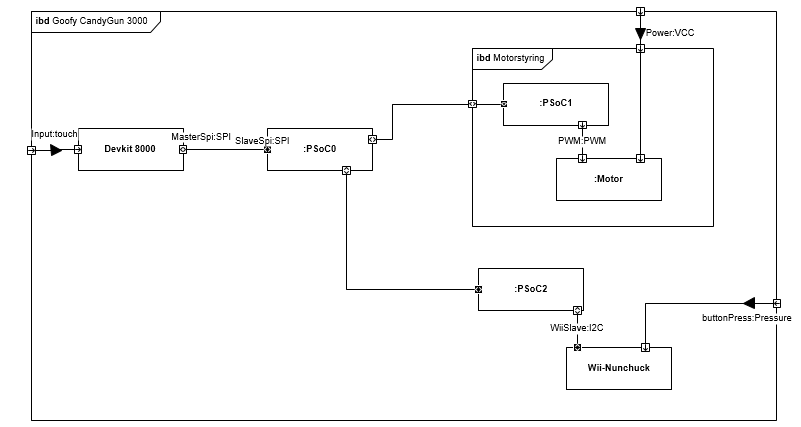
\includegraphics[width=\textwidth]{Systemarkitektur/images/GoofyCandyIBDImageRev2.png}
	\caption{IBD for Candygun 3000}
	\label{fig:IBD}
\end{figure}

\subsection{Signalbeskrivelse}
I signalbeskrivelsen gælder det, at når et signal beskrives som 'højt' opereres der i et spændingsområde på 3.5V til 5V. På samme måde er signaler beskrevet som 'lav' defineret som spændinger indenfor et område fra 0V til 1,5V. Disse spændingsniveauer er defineret  ud fra standarden for CMOS kredse \cite{cmosStandard}.
\begin{longtable}{|>{\hspace{0pt}}p{3cm} | >{\hspace{0pt}}p{3cm} | p{2cm} | p{3cm} |}
	\hline
	\textbf{Blok-navn} & \textbf{Funktionsbeskrivelse} & \textbf{Signaler} & \textbf{Signalbeskrivelse} \\ \hline
	Devkit 8000 & Fungerer som grænseflade mellem bruger og systemet samt SPI master. & masterSPI & Type: SPI \newline Spændingsniveau: 0-5V \newline Hastighed: ?? \newline Beskrivelse: SPI bussen hvori der sendes og modtages data.\\ \cline{3-4}
	& & touch & Type: touch \newline Beskrivelse: Brugertryk på Devkit 8000 touchdisplay. \\ \hline
	PSoC0 & Fungerer som I2C master for PSoC1 og Wii-Nunchuck samt SPI slave til Devkit 8000. & slaveSPI & Type: SPI \newline Spændingsniveau: 0-5V \newline Hastighed: ?? \newline Beskrivelse: SPI bussen hvori der sendes og modtages data.\\ \cline{3-4}
	& & wiiMaster & Type: I2C \newline Spændingsniveau: ?? \newline Hastighed: ?? \newline Beskrivelse: I2C bussen hvor der modtages data fra Nunchuck.\\ \cline{3-4}
	& & motorMaster & Type: I2C \newline Spændingsniveau: 0-5V \newline Hastighed: 100kbit/sekund \newline Beskrivelse: I2C bussen hvor der sendes afkodet Nunchuck data til PSoC1.\\ \hline
	PSoC1 & Modtager nunchuckinput fra PSoC0 og omsætter dataene til PWM signaler. & motorSlave & Type: I2C \newline Spændingsniveau: 0-5V \newline Hastighed: 100kbit/sekund \newline Beskrivelse: Indeholder formatteret Wii-Nunchuck data som omsættes til PWM-signal. \\ \cline{3-4} 
	& & PWM & Type: PWM \newline Frekvens: 22kHz \newline PWM \%: 0-100\% \newline Spændingsniveau: 0-5V \newline Beskrivelse: PWM signal til styring af motorens hastighed. \\ \hline
	Motor & Den enhed der skal bevæge kanonen & PWM & Type: PWM \newline Frekvens: 22kHz \newline PWM\%: 0-100\% \newline Spædingsniveau: 0-5V \newline Beskrivelse: PWM signal til styring af motorens hastighed. \\ \cline{3-4}
	& & motorVoltage & Type: voltage \newline Spændingsniveau: 12V \newline Beskrivelse: Strømforsyning til motoren \\ \hline
	Wii-nunchuck & Den fysiske controller som brugeren styrer kanonen med. & wiiSlave & Type: I2C \newline Spændingsniveau: 0-5V \newline Hastighed: 100kbit/sekund \newline Beskrivelse: Kommunikationslinje mellem PSoC1 og Wii-Nunchuck. \\ \cline{3-4}
	& & userInput & Type: input \newline Beskrivelse: Brugerinput fra Wii-Nunchuck. \\ \hline
	SPI & Denne blok beskriver den ikke-atomiske SPI forbindelse. & MOSI & Type: CMOS \newline Spændingsniveau: 0-5V \newline Hastighed: ?? \newline Beskrivelse: Binært data der sendes fra master til slave. \\ \cline{3-4}
	& & MISO & Type: CMOS \newline Spændingsniveau: 0-5V \newline Hastighed: ?? \newline Beskrivelse: Binært data der sendes fra slave til master. \\ \cline{3-4}
	& & SCLK & Type: CMOS \newline Spændingsniveau: 0-5V \newline Hastighed: ?? \newline Beskrivelse: Clock signalet fra master til slave, som bruges til at synkronisere den serielle kommunikation. \\ \cline{3-4}
	& & SS & Type: CMOS \newline Spændingsniveau: 0-5V \newline Hastighed: ?? \newline  Beskrivelse: Slave-Select, som bruges til at bestemme hvilken slave der skal kommunikeres med. \\ \hline
	I2C & Denne blok beskriver den ikke-atomiske I2C forbindelse. & SDA & Type: CMOS \newline Spændingsniveau: 0-5V \newline Hastighed: ?? \newline Beskrivelse: Databussen mellem I2C masteren og I2C slaver. \\ \cline{3-4}
	& & SCL & Type: CMOS \newline Spændingsniveau: 0-5V \newline Hastighed: ?? \newline Beskrivelse: Clock signalet fra master til lyttende I2C slaver, som bruges til at synkronisere den serielle kommunikation. \\ \hline
	\caption{Tabel med signalbeskrivelse}
\end{longtable}

\section{Software Allokeringsdiagram}
På figur \ref{fig:softwareAllocation} ses et software allokations diagram. Dette diagram danner et overblik over hvilke CPU'er der findes i systemet, og hvilken software der skal allokeres på disse. Følgende applikationsmodeller tager udgangspunkt i softwaren der allokeres i figuren.

\begin{figure}[H]
	\centering
	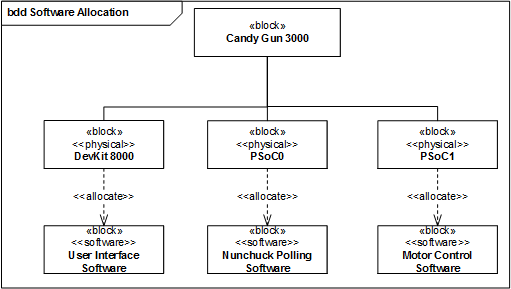
\includegraphics[width=\textwidth]{Systemarkitektur/images/SoftwareAllocation.png}
	\caption{Software allokations diagram}
	\label{fig:softwareAllocation}
\end{figure}

På tabel \ref{tabel:softwareAllocationDescription} er hvert allokeret software komponent beskrevet.

\begin{table}[H]
	\centering
	\begin{tabular}{|ll|}
		\hline
		User Interface Software   & \begin{tabular}[c]{@{}l@{}}Dette allokerede software er brugergrænsefladen\\ som brugeren interagerer med på DevKit8000 touch-skærmen.\end{tabular}                                                  \\
		\rowcolor[HTML]{CBCEFB} 
		Nunchuck Polling Software & \begin{tabular}[c]{@{}l@{}}Dette allokerede software har til ansvar at polle\\ Nunchuck tilstanden og videresende det til\\ PSoC1.\end{tabular}                                                      \\
		Motor Control Software    & \cellcolor[HTML]{FFFFFF}\begin{tabular}[c]{@{}l@{}}Dette allokerede software har til ansvar at\\ bruge den pollede Nunchuck data fra PSoC0\\ til motorstyring samt affyringsmekanismen.\end{tabular} \\ \hline
	\end{tabular}
	\caption{Beskrivelse af den allokerede software}
	\label{tabel:softwareAllocationDescription}
\end{table}

\section{Use Case 1 - Spil Goofy Candy Gun 3000}

Følgende afsnit præsenterer applikationsmodeller relevante til Use Case 1 - Spil Goofy Candy Gun 3000, fordelt over systemets CPU'er.

\begin{figure}[H]
	\centering
	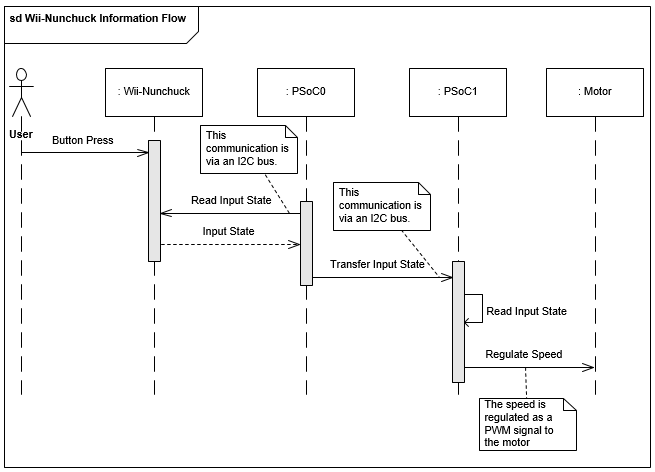
\includegraphics[width=\textwidth]{Systemarkitektur/images/WiiNunchuckSequenceDiagram.png}
	\caption{Overordnet sekvensdiagram for Wii-Nunchuck informations flow}
	\label{fig:WiiNunchuckSequenceDiagram}
\end{figure}

\section{Use Case 2 - Test Kommunikationsprotokoller}

Følgende afsnit præsenterer applikationsmodeller relevante til Use Case 2 - Test Kommunikationsprotokoller, fordelt over systemets CPU'er.

% ---------------Devkit Applikationsmodel-----------------------------
\subsection{Applikationsmodel for User Interface Software}
Sekvensdiagrammet for Devkit 8000 ses på figur \ref{fig:sekvensDevkit}. Kontrolklassen er Test Communication Protocol, er på figurerne er forkortet til TCP. Der er to boundaryklasser, da DevKit 8000 skal håndtere kommunikationen mellem brugeren og PSoC0. Brugeren interagerer via en grafisk brugergrænseflade (GUI). Som det ses af diagrammet initieres testen af brugeren via brugergrænsefladen og derefter er det kontrolklassen, der sørger for, at de forskellige tests bliver sat i gang ved at kommunikere med PSoC0. Når en test er færdiggjort meldes resultatet ud til brugeren via GUI'en.

\begin{figure}[H]
	\centering
	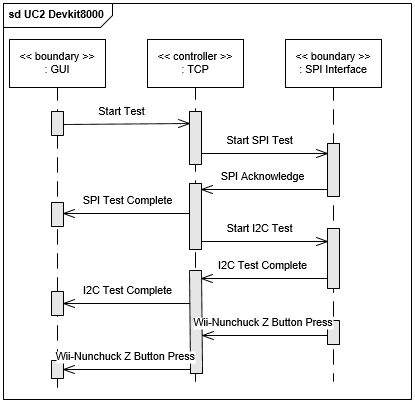
\includegraphics[]{Systemarkitektur/images/DevKit8000SequenceDiagram.png}
	\caption{Sekvensdiagram for Devkit 8000}
	\label{fig:sekvensDevkit}
\end{figure}

Ud fra sekvensdiagrammet for Devkit 8000 er der udledt metoder til klasserne. De udledte metoder ses i klassediagrammet på figur \ref{fig:klasseDevkit}. 

\begin{figure}[H]
	\centering
	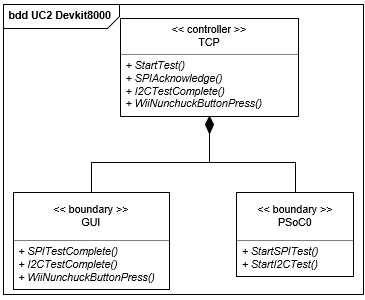
\includegraphics[] {Systemarkitektur/images/DevKit8000ClassDiagram}
	\caption{Klassediagram for Devkit 8000}
	\label{fig:klasseDevkit}
\end{figure}

% ---------------PSoC0 Applikationsmodel-----------------------------
\subsection{Applikationsmodel for Nunchuck Polling Software}
På figur \ref{fig:sekvensPSoC0SPITest}, \ref{fig:sekvensPSoC0I2CTest} og \ref{fig:sekvensPSoC0NunchuckTest} ses sekvensdiagrammer for PSoC0. Sekvensdiagrammerne er blevet opdelt i de 3 tests der gennemføres i use casen; SPI, I2C og Nunchuck kommunikations tests. Kontrolklassen er Test Communication Protocol, hvilket på figurerne er forkortet til TCP. Derudover er der tre boundaryklasser, da PSoC0 skal kommunikere både med Devkit 8000, Nunchucken og PSoC1.

\begin{figure}[H]
	\centering
	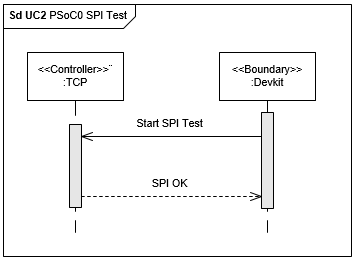
\includegraphics[width=.8\textwidth] {Systemarkitektur/images/SDPSoC0SPITest}
	\caption{Sekvensdiagram for PSoC0 SPI test}
	\label{fig:sekvensPSoC0SPITest}
\end{figure}

På figur \ref{fig:sekvensPSoC0SPITest} ses, at Devkittet sender en besked til kontrolklassen for at påbegynde SPI testen. Når testen er udført, svarer denne med en SPI OK og derved er SPI testen gennemført.

\begin{figure}[H]
	\centering
	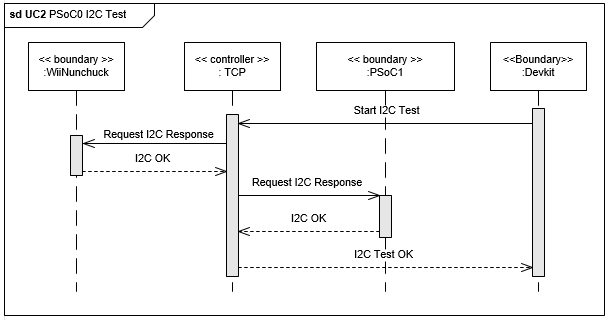
\includegraphics[width=\textwidth] {Systemarkitektur/images/SDPSoC0I2CTest}
	\caption{Sekvensdiagram for PSoC0 I2C test}
	\label{fig:sekvensPSoC0I2CTest}
\end{figure}

På figur \ref{fig:sekvensPSoC0I2CTest} ses, at Devkittet starter I2C testen, ved at sende en besked til kontrolklassen. Kontrolklassen anmoder herefter om svar via I2C nettet fra Nuchucken og PSoC1. Når disse enheder har svaret med et I2C OK er testen gennemført og der sendes besked til Devkittet med en I2C Test OK.

\begin{figure}[H]
	\centering
	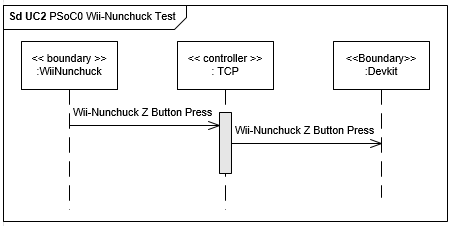
\includegraphics[width=\textwidth] {Systemarkitektur/images/SDPSoC0NunchuckTest}
	\caption{Sekvensdiagram for PSoC0 Nunchuck test}
	\label{fig:sekvensPSoC0NunchuckTest}
\end{figure}

På figur \ref{fig:sekvensPSoC0NunchuckTest} ses sekvensdiagrammet for Wii-Nunchuck testen. Når der sker et tryk sender Nunchucken 'Z' knappens status til kontrolklassen. Herefter videresender kontrolklassen knappens status til Devkittet og derved er testen færdig.\newline

\begin{figure}[H]
	\centering
	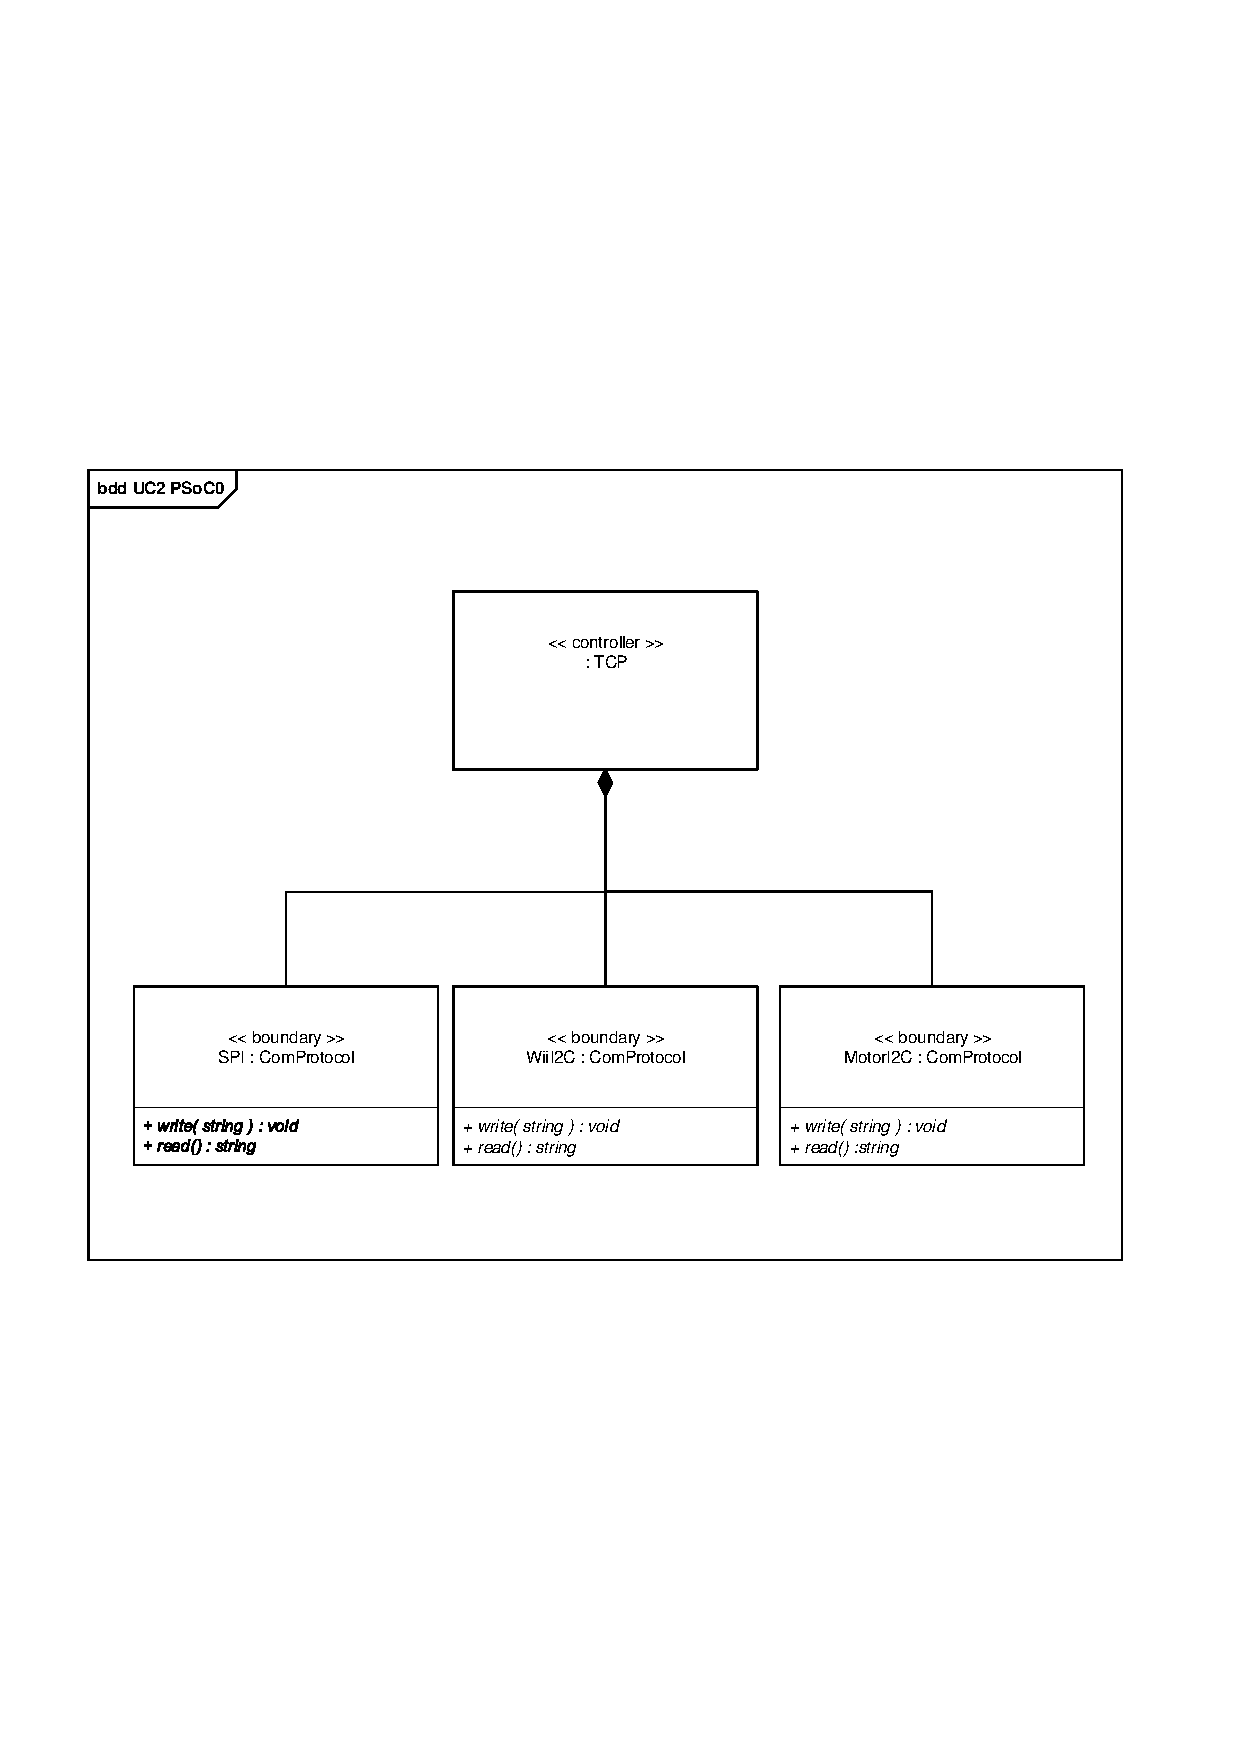
\includegraphics[width=\textwidth]{Systemarkitektur/images/klassediagramPSoC0}
	\caption{Klassediagram for PSoC0}
	\label{fig:klassePSoC0}
\end{figure}

I klassediagrammet på figur \ref{fig:klassePSoC0} ses kontrolklassen og de tre boundaryklasser, som hører til PSoC0. I klasserne er der tilføjet metoder, som er udledt ud fra sekvensdiagrammerne. 

% ---------------PSoC1 Applikationsmodel-----------------------------
\subsection{Applikationsmodel for Motor Control Software}
Sekvensdiagrammet for PSoC1 ses på figur \ref{fig:sekvensPSoC1I2CTest}. Som forrig afsnit er kontrolklassen Test Communication Protocols, hvilket i diagrammet er forkortet til TCP. I dette tilfælde er der kun én boundaryklasse, da PSoC1, i denne use case, kun anvendes til I2C testen og derfor kun skal kommunikere med PSoC0. 

\begin{figure}[H]
	\centering
	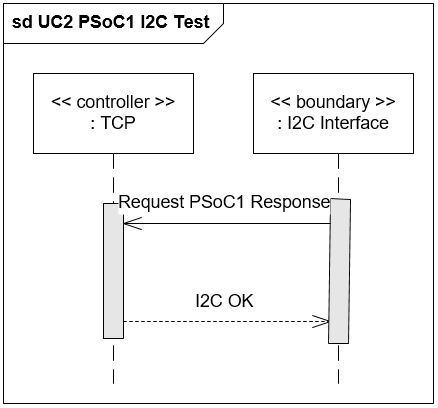
\includegraphics[width=.8\textwidth] {Systemarkitektur/images/SDPSoC1I2CTest}
	\caption{Sekvensdiagram for PSoC1}
	\label{fig:sekvensPSoC1I2CTest}
\end{figure}

På figur \ref{fig:sekvensPSoC1I2CTest} ses, at boundaryklassen, PSoC0, anmoder om respons fra kontrolklassen til at bekræfte om at I2C slaven kan kommunikeres med. Hvis dette er tilfældet sendes der I2C OK tilbage til boundaryklassen.  

\begin{figure}[H]
	\centering
	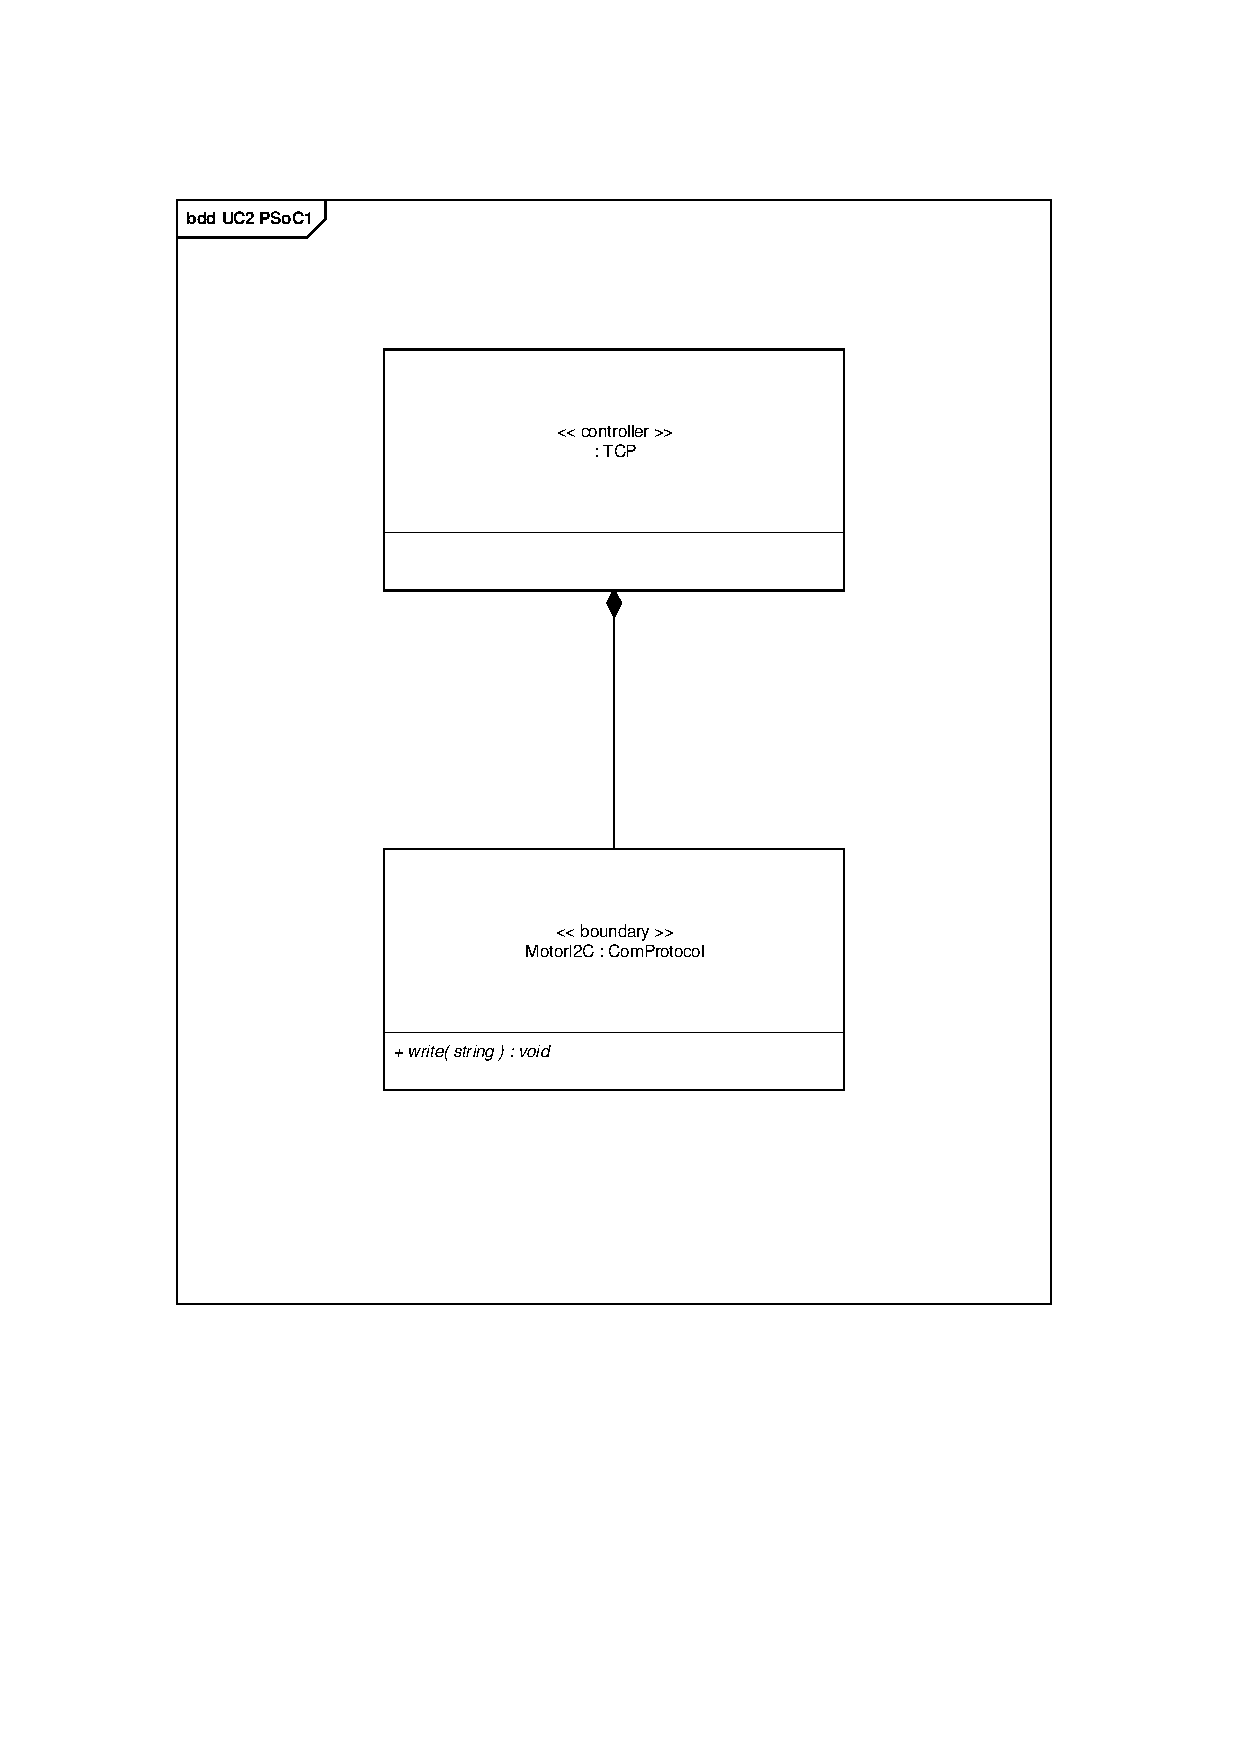
\includegraphics[width=.5\textwidth]{Systemarkitektur/images/klassediagramPSoC1}
	\caption{Klassediagram for PSoC1}
	\label{fig:klassePSoC1}
\end{figure}

Fra sekvensdiagrammet på figur \ref{fig:sekvensPSoC1I2CTest} udledes et klassediagram som ses foroven i figur \ref{fig:klassePSoC1}.

\section{Kommunikationsprotokoller}
\label{afsnit:kommunikationsprotokoller}
I dette afsnit beskrives de kommunikationsprotokoller der anvendes til at sende data mellem systemets komponenter på de anvendte bustyper - I2C og SPI. På figur \ref{fig:kommunikationsOverblik} ses hvilke bustyper der anvendes mellem systemets komponenter. 

\begin{figure}[H]
	\centering
	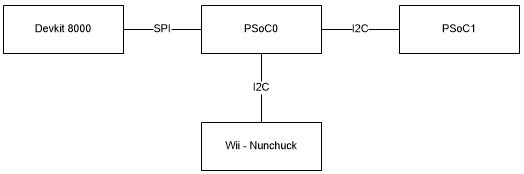
\includegraphics[width=\textwidth] {Systemarkitektur/images/anvendtebustyper}
	\caption{Forbindelser mellem systemets komponenter}
	\label{fig:kommunikationsOverblik}
\end{figure}

\subsection{SPI Protokol}
\label{afsnit:spiprotokol}
Til kommunikation mellem Devkittet og PSoC0 anvendes der \textit{Serial Parallel Interface (SPI)}. SPI-forbindelsen består af fire signaler. Et af signalerne er \textit{slave select} (SS). Det muliggør kommunikation med flere slaver. Selve dataen sendes via signalerne \textit{Master Out Slave In} (MOSI) og \textit{Master In Slave Out} (MISO). Det foregår ved \textit{Full Duplex}, hvor der altid sendes i begge retninger på én gang. Hvis der kun ønskes at sende i én retning, kan der sendes 0'er i den anden retning. Derudover er der en \textit{Clock} (SCLK), som sørger for at kommunikationen er synkron. I forhold til timing er det vigtigt, at både master og slave anvender samme \textit{Timing Mode}, som styres af to bit, \textit{SPI Clock Polarity Bit} (CPOL), som bestemmer om clock'en starter højt eller lavt, og \textit{SPI Clock Phase Bit} (CPHA), som afgør om data samples på clock'ens rising- eller falling edge. I dette projekt anvendes \textit{Timing Mode 3}, hvor clock'en starter høj og sampler på rising edge. \\
De kommandoer, der i projektet sendes via SPI, består af 8 bit. \\
På tabel \ref{tabel:spiKommandoType} ses SPI-protokollen. Til venstre på tabellen ses navnet på de kommandoer, der sendes. Alle kommandoer med "TEST" i navnet sendes fra Devkit8000 til PSoC0 via MOSI. De resterende kommandoer er svar på de forskellige tests, som sendes via MISO fra PSoC0 til Devkit8000. Det er værd at lægge mærke til, at det er bevidst, at der ikke er en kommando for SPI\_FAIL. Da SPI-forbindelsen ikke testes på PSoC0, men ved at PSoC0 sender \textit{SPI\_OK} tilbage til Devkit8000 via SPI-forbindelsen. Dermed kan det først afgøres om SPI-forbindelsen fungerer korrekt, når Devkit8000, modtager (eller ikke modtager) succes-beskeden fra PSoC0. \\


\begin{table}[H]
	\centering
	\resizebox{\textwidth}{!}{%
		\begin{tabular}{llll}
			\hline
			\multicolumn{1}{|l|}{Kommandotype}                                & \multicolumn{1}{l|}{Beskrivelse}                        & \multicolumn{1}{l|}{Binær Værdi} & \multicolumn{1}{l|}{Hex Værdi} \\ \hline
			\rowcolor[HTML]{CBCEFB} 
			{\color[HTML]{000000} START\_SPI\_TEST}                           & {\color[HTML]{000000} Sætter PSoC0 i 'SPI-TEST' mode}   & 1111 0001                        & 0xF1                           \\
			START\_I2C\_TEST                                                  & Sætter PSoC0 i 'I2C-TEST' mode                          & 1111 0010                        & 0xF2                           \\
			\rowcolor[HTML]{CBCEFB} 
			\begin{tabular}[c]{@{}l@{}}START\_NUN-\\ CHUCK\_TEST\end{tabular} & Sætter PSoC0 i 'NUNCHUCK-TEST' mode                     & 1111 0011                        & 0xF3                           \\
			SPI\_OK                                                           & Signalerer at SPI-testen blev gennemført uden fejl      & 1101 0001                        & 0xD1                           \\
			\rowcolor[HTML]{CBCEFB} 
			I2C\_OK                                                           & Signalerer at I2C-testen blev gennemført uden fejl      & 1101 0010                        & 0xD2                           \\
			I2C\_FAIL                                                         & Signalerer at der skete fejl under I2C-testen           & 1100 0010                        & 0xC2                           \\
			\rowcolor[HTML]{CBCEFB} 
			NUNCHUCK\_OK                                                      & Signalerer at NUNCHUCK-testen blev gennemført uden fejl & 1101 0011                        & 0xD3                           \\
			NUNCHUCK\_FAIL                                                    & Signalerer at der skete fejl under NUNCHUCK-testen      & 1100 0011                        & 0xC3                          
		\end{tabular}
	}
	\caption{Kommandotyper der anvendes ved SPI kommunikation}
	\label{tabel:spiKommandoType}
\end{table}

For at aflæse en besked fra SPI-slaven, skal slaven først klargøre dens SPI-transfer buffer. Dette gøres ved, at SPI-masteren sender en commandotype til slaven, som derefter tolker kommandotypen, og eksekverer kommandoen, hvor SPI-transfer bufferen bliver sat. Imens dette sker, venter SPI-masteren i et bestemt stykke tid, for at sikre at transfer-bufferen når at blive sat. På figur \ref{figure:SDSpiReadSlave} ses et sekvensdiagram der illustrerer dette. 

\begin{figure}[H]
	\centering
	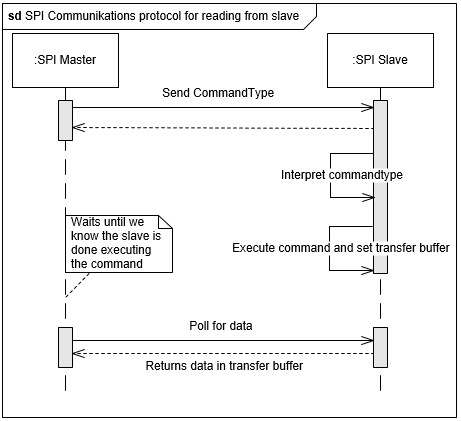
\includegraphics[]{SystemArkitektur/images/SDSpiSlaveRead}
	\caption{Sekvensdiagram for at læse fra SPI-slaven}
	\label{figure:SDSpiReadSlave}
\end{figure}


\subsection{I2C Protokol}
\label{afsnit:I2CProtokol}

I2C\cite{I2C} er en bus bestående af to ledninger. Den ene ledning bruges som databus og navngives \textit{Serial Data Line} (SDA). Den anden ledning bruges til clock signalet, der synkroniserer kommunikationen, og navngives \textit{Serial Clock Line} (SCL). Enheder på I2C bussen gør brug af et master-slave forhold til at sende og læse data. En fordel ved I2C bussen er at netværket kan bestå af multiple masters og slaver, hvilket udnyttes i dette system da tre I2C komponenter skal sende data mellem hinanden.

I2C gør brug af en integreret protokol der anvender adressering af hardware-enheder for at identificere hvilken enhed der kommunikeres med. På tabel \ref{table:I2CAddress} ses addresserne tildelt systemets PSoCs.

\begin{table}[H]
	\centering
	\begin{tabular}{lllllllll}
		\hline
		\multicolumn{1}{|l|}{I2C Adresse bits} & 7                        & 6                        & 5                        & 4 & 3 & 2 & \multicolumn{1}{l|}{1} & \multicolumn{1}{l|}{0 (R/W)} \\ \hline
		\rowcolor[HTML]{CBCEFB} 
		{\color[HTML]{000000} PSoC0}           & {\color[HTML]{000000} 0} & {\color[HTML]{000000} 0} & {\color[HTML]{000000} 0} & 1 & 0 & 0 & 0                      & 0/1                          \\
		PSoC1                                  & 0                        & 0                        & 0                        & 1 & 0 & 0 & 1                      & 0/1                         
	\end{tabular}
	\caption{Adresser der anvendes på I2C bussen}
	\label{table:I2CAddress}
\end{table}

Den integrerede I2C protokol sender data serielt i pakker af 8-bit (1 byte). På figur \ref{fig:I2CTimingDiagram} ses et timing diagram for aflæsning af 1 byte. Figuren er et udsnit fra databladet for en LM75, der anvender fire faste addressebits, tre vilkårlige bit og en read/write bit. Her ses at transmissionen af data begynder med en addresse-byte til slaven efterfulgt en acknowledge til masteren og herefter sendes en data-byte. 

\begin{figure}[H]
	\centering
	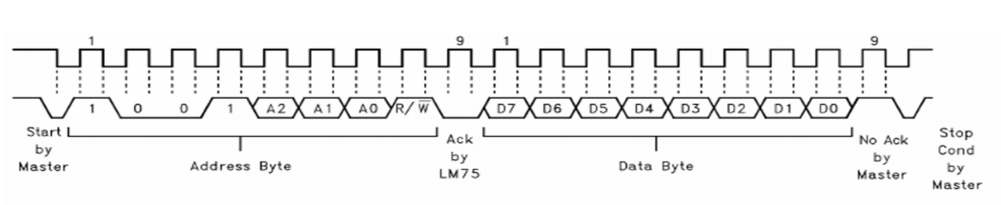
\includegraphics[width=\textwidth] {Systemarkitektur/images/I2CTimingDiagram}
	\caption{Timing Diagram af 1-byte I2C aflæsning}
	\label{fig:I2CTimingDiagram}
\end{figure}

Goofy candygun gør brug af I2C protokollen via PSoC's I2C \textit{Application Programming Interface} (API). Ved brug af denne API er der blevet udviklet en kommunikationsprotokol mellem systemets PSoCs, som gør det muligt at sende kommandoer og data.

Da I2C dataudveksling sker bytevist, er kommunikations protokollen opbygget ved, at kommandoens type indikeres af den første modtagne byte. Herefter følger \textit{N}-antal bytes som er kommandoens tilhørende data. \textit{N} er et vilkårligt heltal og bruges i dette afsnit når der refereres til en mængde data-bytes der sendes med en kommandotype.

Kommandoens type definerer antallet af databytes modtageren skal forvente og hvordan disse skal fortolkes. På figur \ref{fig:I2CProtokolEksempel} ses et sekvensdiagram der, med pseudo-kommandoer, demonstrerer forløbet mellem en I2C afsender og modtager ved brug af kommunikations protokollen.

\begin{figure}[H]
	\centering
	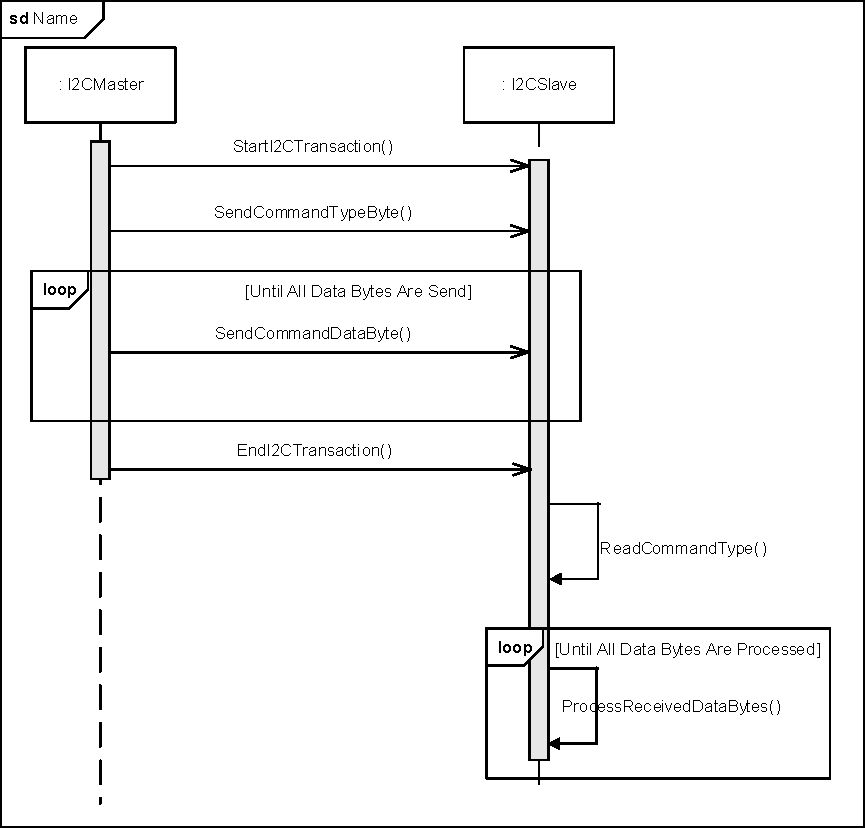
\includegraphics[width=\textwidth] {Systemarkitektur/images/I2CProtocol}
	\caption{Eksempel af I2C Protokol Forløb}
	\label{fig:I2CProtokolEksempel}
\end{figure}

På figur \ref{fig:I2CProtokolEksempel} ses at afsenderen først starter en I2C transaktion, hvorefter typen af kommando sendes som den første byte. Efterfølgende sendes \textit{N} antal bytes, afhængig af hvor meget data den givne kommandotype har brug for at sende. Efter afsluttet I2C transaktion læser I2C modtageren typen af kommando, hvor den herefter kan fortolke \textit{N} antal modtagne bytes afhængig af den modtagne kommandotype.

På tabel \ref{table:I2CKommandoer} ses de definerede kommandotyper og det tilsvarende antal af bytes der sendes ved dataveksling.

\begin{table}[H]
	\centering
	\resizebox{\textwidth}{!}{
		\begin{tabular}{lllll}
			\hline
			\multicolumn{1}{|l|}{Kommandotype}    & \multicolumn{1}{l|}{Beskrivelse}                                            & \multicolumn{1}{l|}{Binær Værdi} & \multicolumn{1}{l|}{Hex Værdi} & \multicolumn{1}{l|}{Data Bytes}                                                                                         \\ \hline
			\rowcolor[HTML]{CBCEFB} 
			{\color[HTML]{000000} NunchchuckData} & {\color[HTML]{000000} Indeholder aflæst data fra Wii Nunchuck controlleren} & 0010 1010                        & 0xA2                           & \begin{tabular}[c]{@{}l@{}}Byte \#1 Analog X-værdi\\ Byte \#2 Analog Y-værdi\\ Byte \#3 Analog Buttonstate\end{tabular} \\
			I2CTestRequest                        & Anmoder PSoC0 om at starte I2C-kommunikations test                          & 0010 1001                        & 0x29                           & Ingen databyte                                                                                                          \\
			\rowcolor[HTML]{CBCEFB} 
			I2CTestAck                            & Anmodning om at få en I2C OK besked fra I2C enhed                           & 0010 1000                        & 0x28                           & Ingen databyte                                                                                                         
		\end{tabular}
	}
	\caption{Kommandotyper der anvendes ved I2C kommunikation}
	\label{table:I2CKommandoer}
\end{table}

Kolonnerne "Binær Værdi" og "Hex Værdi" i tabel \ref{table:I2CKommandoer} viser kommandotypens unikke tal-ID i både binær- og hexadecimalform. Denne værdi sendes som den første byte, for at identificere kommandotypen. 




